% TikZ source of Fig. 2 (compile separately with pdflatex; the manuscript includes fig2_pipeline.pdf)
\documentclass[tikz,border=2pt]{standalone}
\usepackage{mathptmx}
\usepackage{amsmath,amssymb}
\usetikzlibrary{positioning,arrows.meta,calc}
\definecolor{cdata}{RGB}{232,232,232}
\definecolor{cscore}{RGB}{214,222,248}
\definecolor{csite}{RGB}{212,240,212}
\definecolor{ccert}{RGB}{248,214,214}
\definecolor{cw}{RGB}{252,228,196}
\definecolor{cann}{RGB}{176,96,0}
\begin{document}
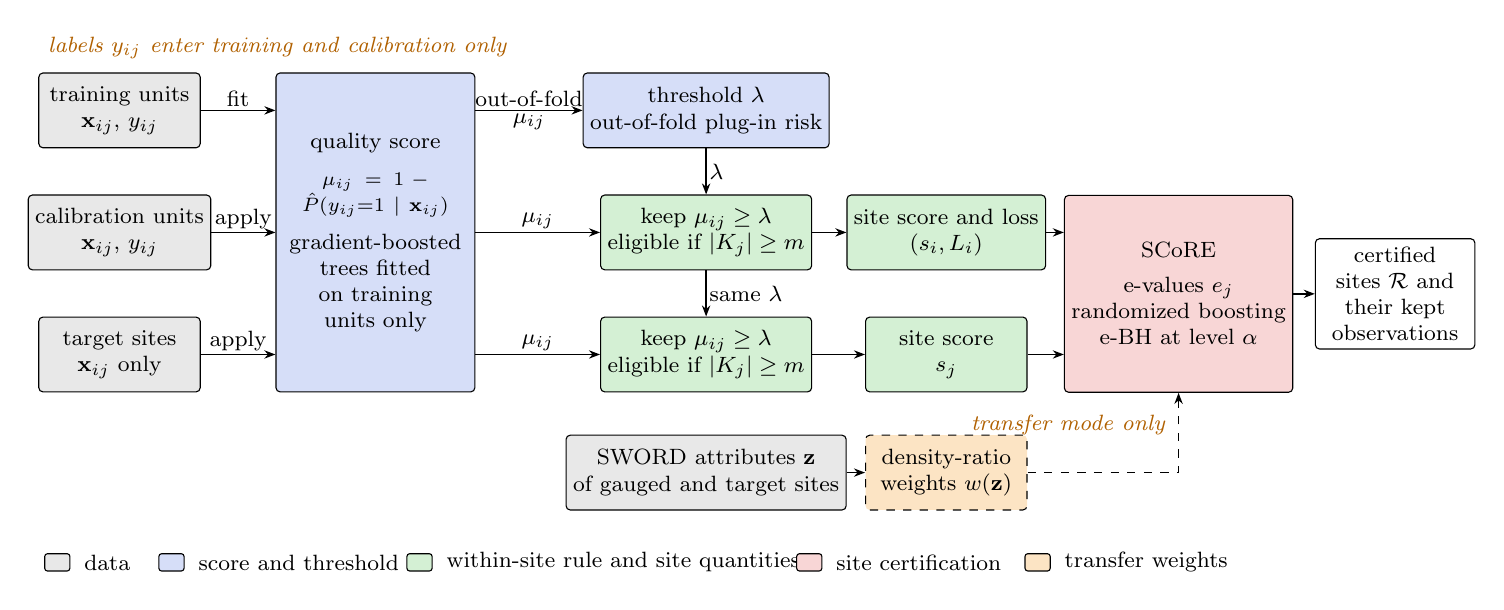
\begin{tikzpicture}[font=\footnotesize, >={Stealth[length=4pt]},
  box/.style={draw, rounded corners=1.5pt, align=center, inner sep=2.5pt, minimum height=0.95cm},
  line/.style={->, line width=0.55pt},
  lab/.style={font=\footnotesize, inner sep=1pt}]
\node[box, fill=cdata, minimum width=2.05cm] (tr) at (0, 1.55) {training units\\ $\mathbf{x}_{ij},\, y_{ij}$};
\node[box, fill=cdata, minimum width=2.05cm] (ca) at (0, 0.0) {calibration units\\ $\mathbf{x}_{ij},\, y_{ij}$};
\node[box, fill=cdata, minimum width=2.05cm] (ta) at (0, -1.55) {target sites\\ $\mathbf{x}_{ij}$ only};
\node[box, fill=cscore, text width=2.35cm, minimum height=4.05cm] (sc) at (3.25, 0.0) {quality score\\[4pt] {\scriptsize $\mu_{ij} = 1 - \hat{P}(y_{ij}{=}1 \mid \mathbf{x}_{ij})$}\\[4pt] gradient-boosted trees fitted on training units only};
\node[box, fill=cscore, minimum width=2.6cm] (la) at (7.45, 1.55) {threshold $\lambda$\\ out-of-fold plug-in risk};
\node[box, fill=csite, minimum width=2.6cm] (r2) at (7.45, 0.0) {keep $\mu_{ij} \geq \lambda$\\ eligible if $|K_j| \geq m$};
\node[box, fill=csite, minimum width=2.6cm] (r3) at (7.45, -1.55) {keep $\mu_{ij} \geq \lambda$\\ eligible if $|K_j| \geq m$};
\node[box, fill=csite, minimum width=2.05cm] (s2) at (10.5, 0.0) {site score and loss\\ $(s_i, L_i)$};
\node[box, fill=csite, minimum width=2.05cm] (s3) at (10.5, -1.55) {site score\\ $s_j$};
\node[box, fill=cdata, minimum width=2.6cm] (z) at (7.45, -3.05) {SWORD attributes $\mathbf{z}$\\ of gauged and target sites};
\node[box, fill=cw, dashed, minimum width=2.05cm] (w) at (10.5, -3.05) {density-ratio\\ weights $w(\mathbf{z})$};
\node[box, fill=ccert, minimum width=2.3cm, minimum height=2.5cm] (ce) at (13.45, -0.78) {SCoRE\\[3pt] e-values $e_j$\\ randomized boosting\\ e-BH at level $\alpha$};
\node[box, fill=white, text width=1.85cm, minimum height=1.4cm] (out) at (16.2, -0.78) {certified sites $\mathcal{R}$ and their kept observations};
\draw[line] (tr.east) -- node[lab, above] {fit} (tr.east -| sc.west);
\draw[line] (ca.east) -- node[lab, above] {apply} (ca.east -| sc.west);
\draw[line] (ta.east) -- node[lab, above] {apply} (ta.east -| sc.west);
\draw[line] (sc.east |- la.west) -- node[lab, above] {out-of-fold} node[lab, below] {$\mu_{ij}$} (la.west);
\draw[line] (sc.east |- r2.west) -- node[lab, above] {$\mu_{ij}$} (r2.west);
\draw[line] (sc.east |- r3.west) -- node[lab, above] {$\mu_{ij}$} (r3.west);
\draw[line] (la.south) -- node[lab, right] {$\lambda$} (r2.north);
\draw[line] (r2.south) -- node[lab, right] {same $\lambda$} (r3.north);
\draw[line] (r2.east) -- (s2.west);
\draw[line] (r3.east) -- (s3.west);
\draw[line] (z.east) -- (w.west);
\draw[line] (s2.east) -- (s2.east -| ce.west);
\draw[line] (s3.east) -- (s3.east -| ce.west);
\draw[line, dashed] (w.east) -| node[lab, pos=0.8, left, xshift=-3pt, text=cann] {\textit{transfer mode only}} (ce.south);
\draw[line] (ce.east) -- (out.west);
\node[font=\footnotesize\itshape, text=cann, anchor=south west] at (-1.03, 2.08) {labels $y_{ij}$ enter training and calibration only};
\begin{scope}[shift={(-0.95,-4.3)}, every node/.style={font=\footnotesize, anchor=west}]
\foreach \c/\t/\xx in {cdata/data/0, cscore/score and threshold/1.45, csite/within-site rule and site quantities/4.6, ccert/site certification/9.55, cw/transfer weights/12.45}{
  \draw[fill=\c, rounded corners=1pt] (\xx,0) rectangle ++(0.32,0.22);
  \node at (\xx+0.38,0.11) {\t};
}
\end{scope}
\end{tikzpicture}
\end{document}
